\documentclass{article}
\usepackage[utf8]{inputenc}
\usepackage{graphicx}
\usepackage{geometry}
\newgeometry{vmargin={15mm},hmargin={12mm,17mm}}   % set the margins
\title{Exercise\_01}
\author{Ramona Walker, Dominik Johann Arnold, Mark Woolley, Otto Buck}
\date{November 2022}

\begin{document}

\maketitle

\section{CRC Cards}
These are the CRC Cards as we created them when we started. \\
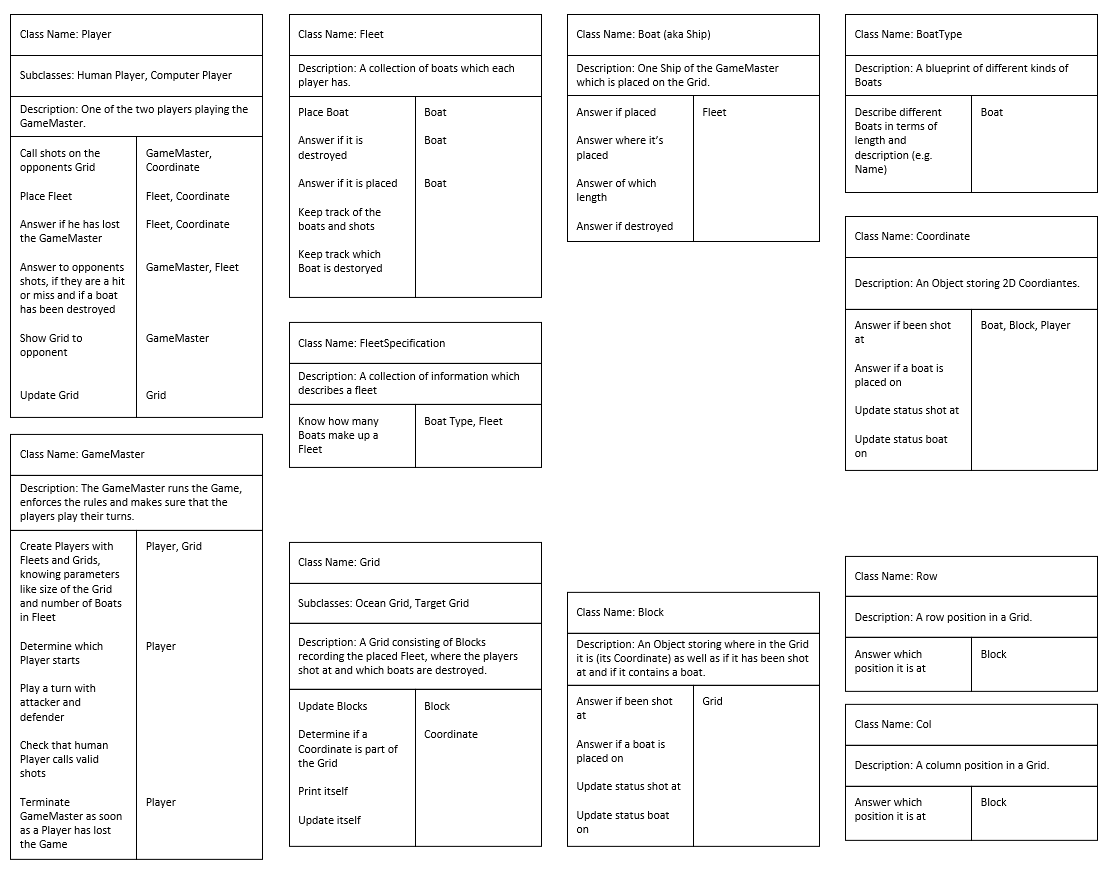
\includegraphics[width = \linewidth]{images/CRC cards.png}
\newpage




\section{Following the Responsibility Driven Design, describe the main classes you designed to be your project in terms of responsibilities and collaborations.}

\begin{itemize}
    \item \textbf{Game / GameMaster}\\
    GameMaster makes sure the game is played according to the rules and has two players. The class is responsible for stopping the game when it's over.\\
    \textbf{Responsibilities}: Initialize the game and ensure the correct execution of the game rules. Determine the starting player and make sure the game ends when a player has lost.\\
    \textbf{Collaborations}: Mainly interact with the \textit{Players} of which the game consists of. Interact directly with the Players \textit{Grid} when the GameMaster must print the state of the game. GameMaster uses \textit{Coordinates} to play a turn.
\\
    \item \textbf{Player (Subclass PlayerHuman, PlayerComputer)}\\
    A Player has ONE Grid and ONE Fleet. He collaborates with the GameMaster by declaring and receiving shots. He collaborates with his Fleet and Grid during placement of Boats and while declaring and receiving shots.\\
    \textbf{Note:} Difference between Human and Computer is only how they place their Fleet and how they call shots. Computer is randomized (or any strategy really), Human is via user input.\\
    \textbf{Responsibilities:} Must place his Fleet, which leads to Boats being placed. Must be able to call valid shots for the other player as well as receive them from the other player (via GameMaster). Simultaneously, whenever the Fleet is changed or shots are recorded, the player must update his Fleet and Grid accordingly. Furthermore, the player must be able to provide his up-to-date Grid to the GameMaster and he must be able to declare whether he has lost the game.\\
    \textbf{Collaborations:} With the \textit{GameMaster} when supplying the Grid. With the \textit{Fleet} in all actions regarding placement and shots receiving. When placing the fleet, \textit{Boat} in Fleet is called. With the \textit{Grid} during all the actions which lead to the player updating his Grid. A list of \textit{Coordinates} is used to store received and taken shots.
    
    \item \textbf{Fleet}\\
    A Fleet is a collection of Boats and keeps track of placed and destroyed Boats. The specification of the collection is set in the game rules.\\
    \textbf{Responsibilities:} At any point declare if the whole Fleet is destroyed. The Fleet can receive a shot and declare if any Boat is hit. Must be able to place a Boat when given a list of Coordinates and must be able to tell for a given list of Coordinates if there is an overlap in boats (e.g. if there is a boat already).\\
    \textbf{Collaborations:} With the \textit{Boat} and \textit{Coordinate} when a Boat is placed and when the status (destroyed) is determined. With \textit{FleetSpecification} to receive the specific boats it consists of.
    
    \item \textbf{Grid}\\
    A Grid is a collection of Blocks, given the size of the game rules. It must be able to print itself as either target or ocean grid and needs to update its Blocks according to different events.\\
    \textbf{Responsibilities:} The Grid must provide a printing method as either a target or ocean grid. It must be able to record and remember shots taken at it and boats placed on it.\\
    \textbf{Collaborations:} With the \textit{Block} whenever a block needs to get updated. The Player will ask the Grid to update for different events. The Grid will pass on this Information to the correct Block. Therefore it also needs to collaborate with \textit{Coordinate}. To print it needs to collaborate with \textit{GameUtils}. (Changing integers to coordinates and getting game size.)
    
    \item \textbf{Block}\\
    A Block is the elementary unit of the grid. Each block has a position in the grid in form of a Coordinate. Furthermore, it knows its state regarding if it has been shot at, it has a boat placed on itself, if it should act as destroyed and what the printing character is.\\
    \textbf{Note}: Not all states are important for both printing options.\\
    \textbf{Responsibilities}: Know and update the status regarding shot at, boat placed on, destroyed status and what kind of character to print if a boat is on there. Need to be able to be called to change any state.\\
    \textbf{Collaborations}: With the \textit{Coordinate} to store its location.
    
    \item \textbf{Coordinate}\\
    The Coordinate is the fundamental building block of the whole game and is used through all classes. It provides a common language for positions which make up Blocks, shots, and anything else in the game. It can also convert between internal integer representation of rows and columns and the external representation (e.g. A2)\\
    \textbf{Responsibilities}: Be able to tell the position in a 2D plane with row and columns numbers. Must be able to print itself either in integer representation or in external representation\\
    \textbf{Collaborations}: With \textit{GameUtils} to convert integer-representation to letter-representation.
    
    \item \textbf{FleetSpecification}\\
    This class is a lookup artifact which specifies what number of different BoatTypes a Fleet consists of.\\
    \textbf{Responsibilities}: Know the exact number of BoatTypes which make up a Fleet. Give that Information to Fleet.\\
    \textbf{Collaborations}: With \textit{Boattype} to define what boats are in a fleet.
    
    \item \textbf{BoatType}\\
    This class describes the different types of Boats that exist in terms of name, description, and length.\\
    \textbf{Responsibilities}: Know what kind of Boats exist and provide this information.\\
    \textbf{Collaborations}: none
\end{itemize}




\newpage
\section{Why do you consider the other classes as less important? Following the Responsibility Driven Design, reflect if some of those non-main classes have similar/little responsibility and could be changed, merged, or removed.}

\begin{itemize}
    \item \textbf{OceanGrid, TargetGrid}\\
    We realized that the distinction between two different grids is superfluous. It's enough that each Player only has one Grid and the Grid itself must be able to present itself as either target or ocean grid.
    
    \item \textbf{Row / Column Types}\\
    We decided to not use enum types to depict rows and columns and use simple integers instead. Reasoning: The most natural way to describe rows and columns as coordinates are in fact integers, not enum types.
    
    \item \textbf{FleetSpecification}\\
    The FleetSpecificaiton could also be set in the game rules, but we decided to make it a dedicated enum type. We think that it makes the organization of the code cleaner.

\end{itemize}




\newpage
\section{Draw the class diagram of the aforementioned main elements of your game.}
\begin{figure}[h]
\centering
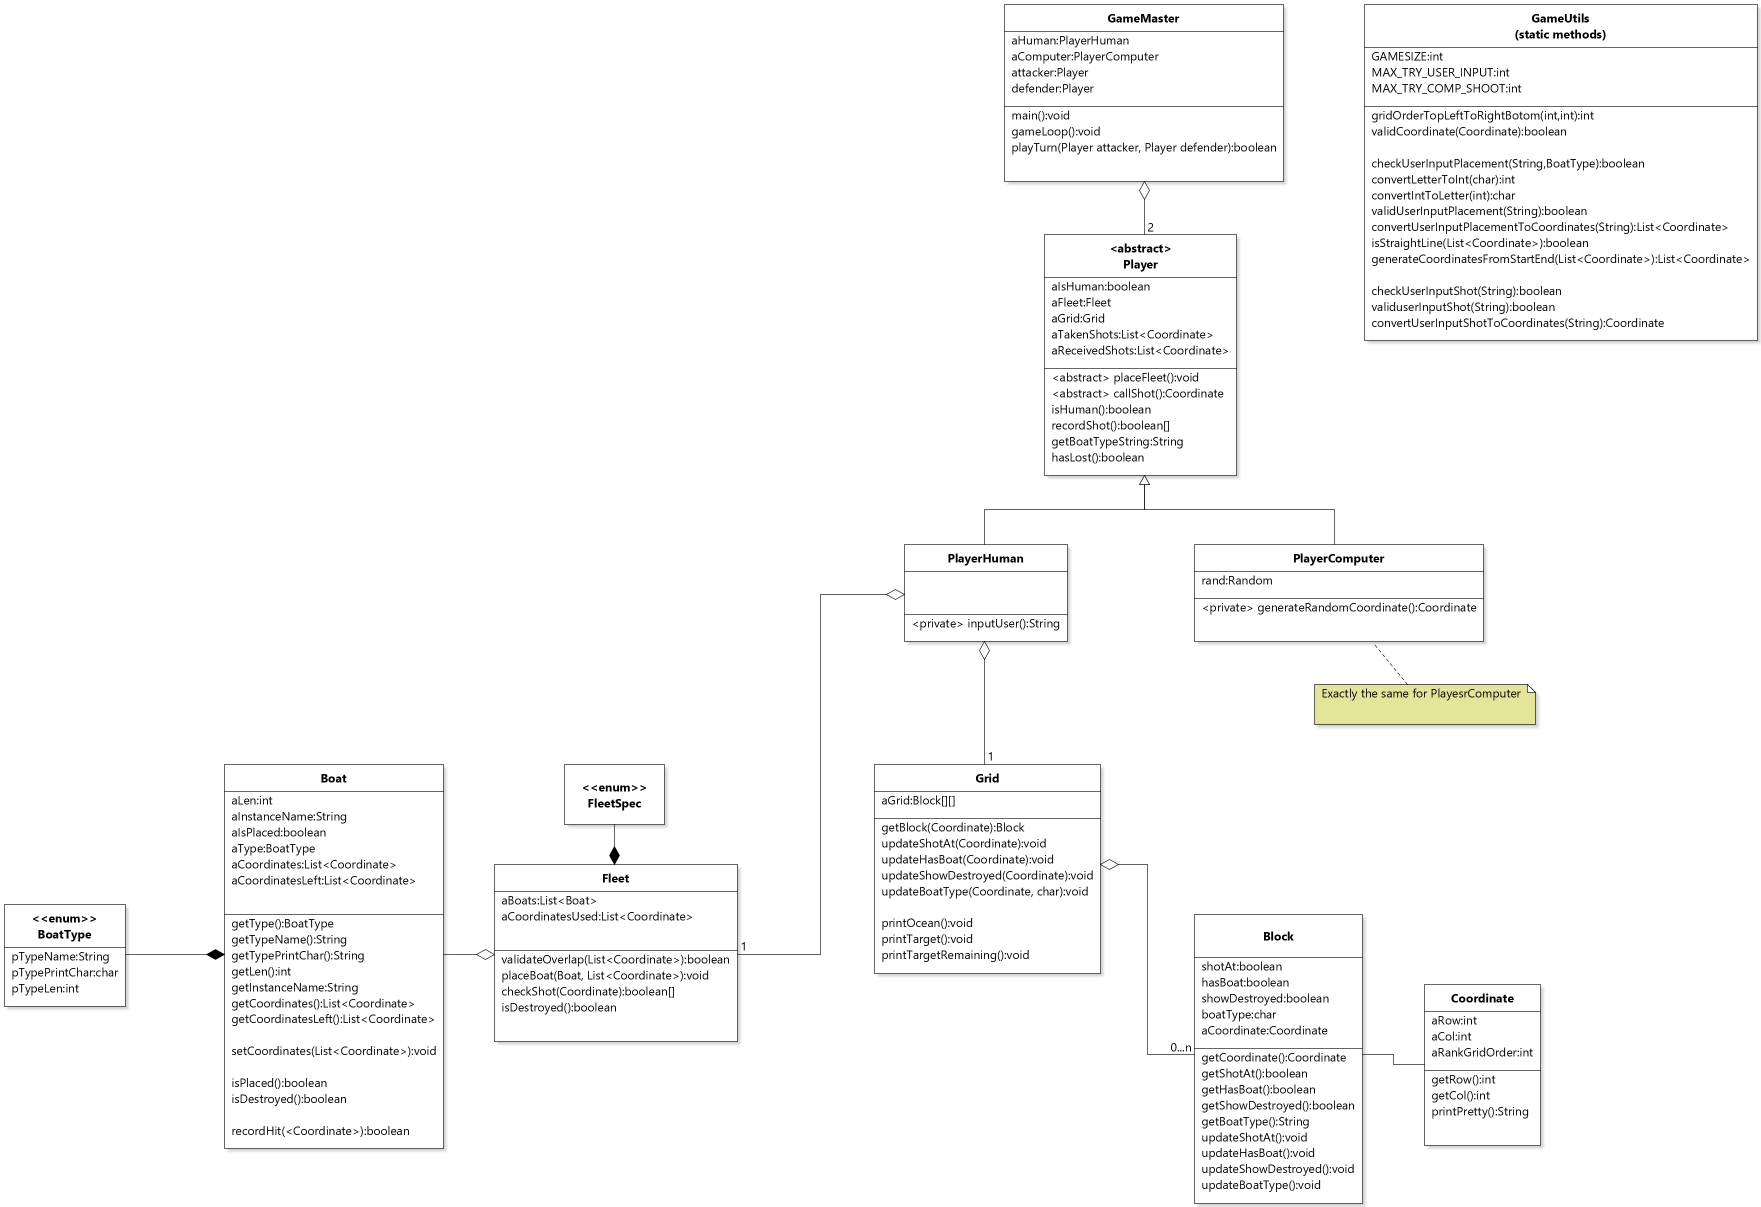
\includegraphics[width = \linewidth]{images/class_diagram.png}
\caption{Class diagram}
\end{figure}


\newpage
\section{Draw an object diagram to show the main elements of your game in a step of the game of your choosing.}
This section includes two object diagrams. The first is a complete state of the game, including all Coordinate objects. The second one depicts the exact same situation, but for clarity leaves out all Coordinate objects. This is meant to help understanding the major elements without cluttering the diagram.  

\begin{figure}[h]
\centering
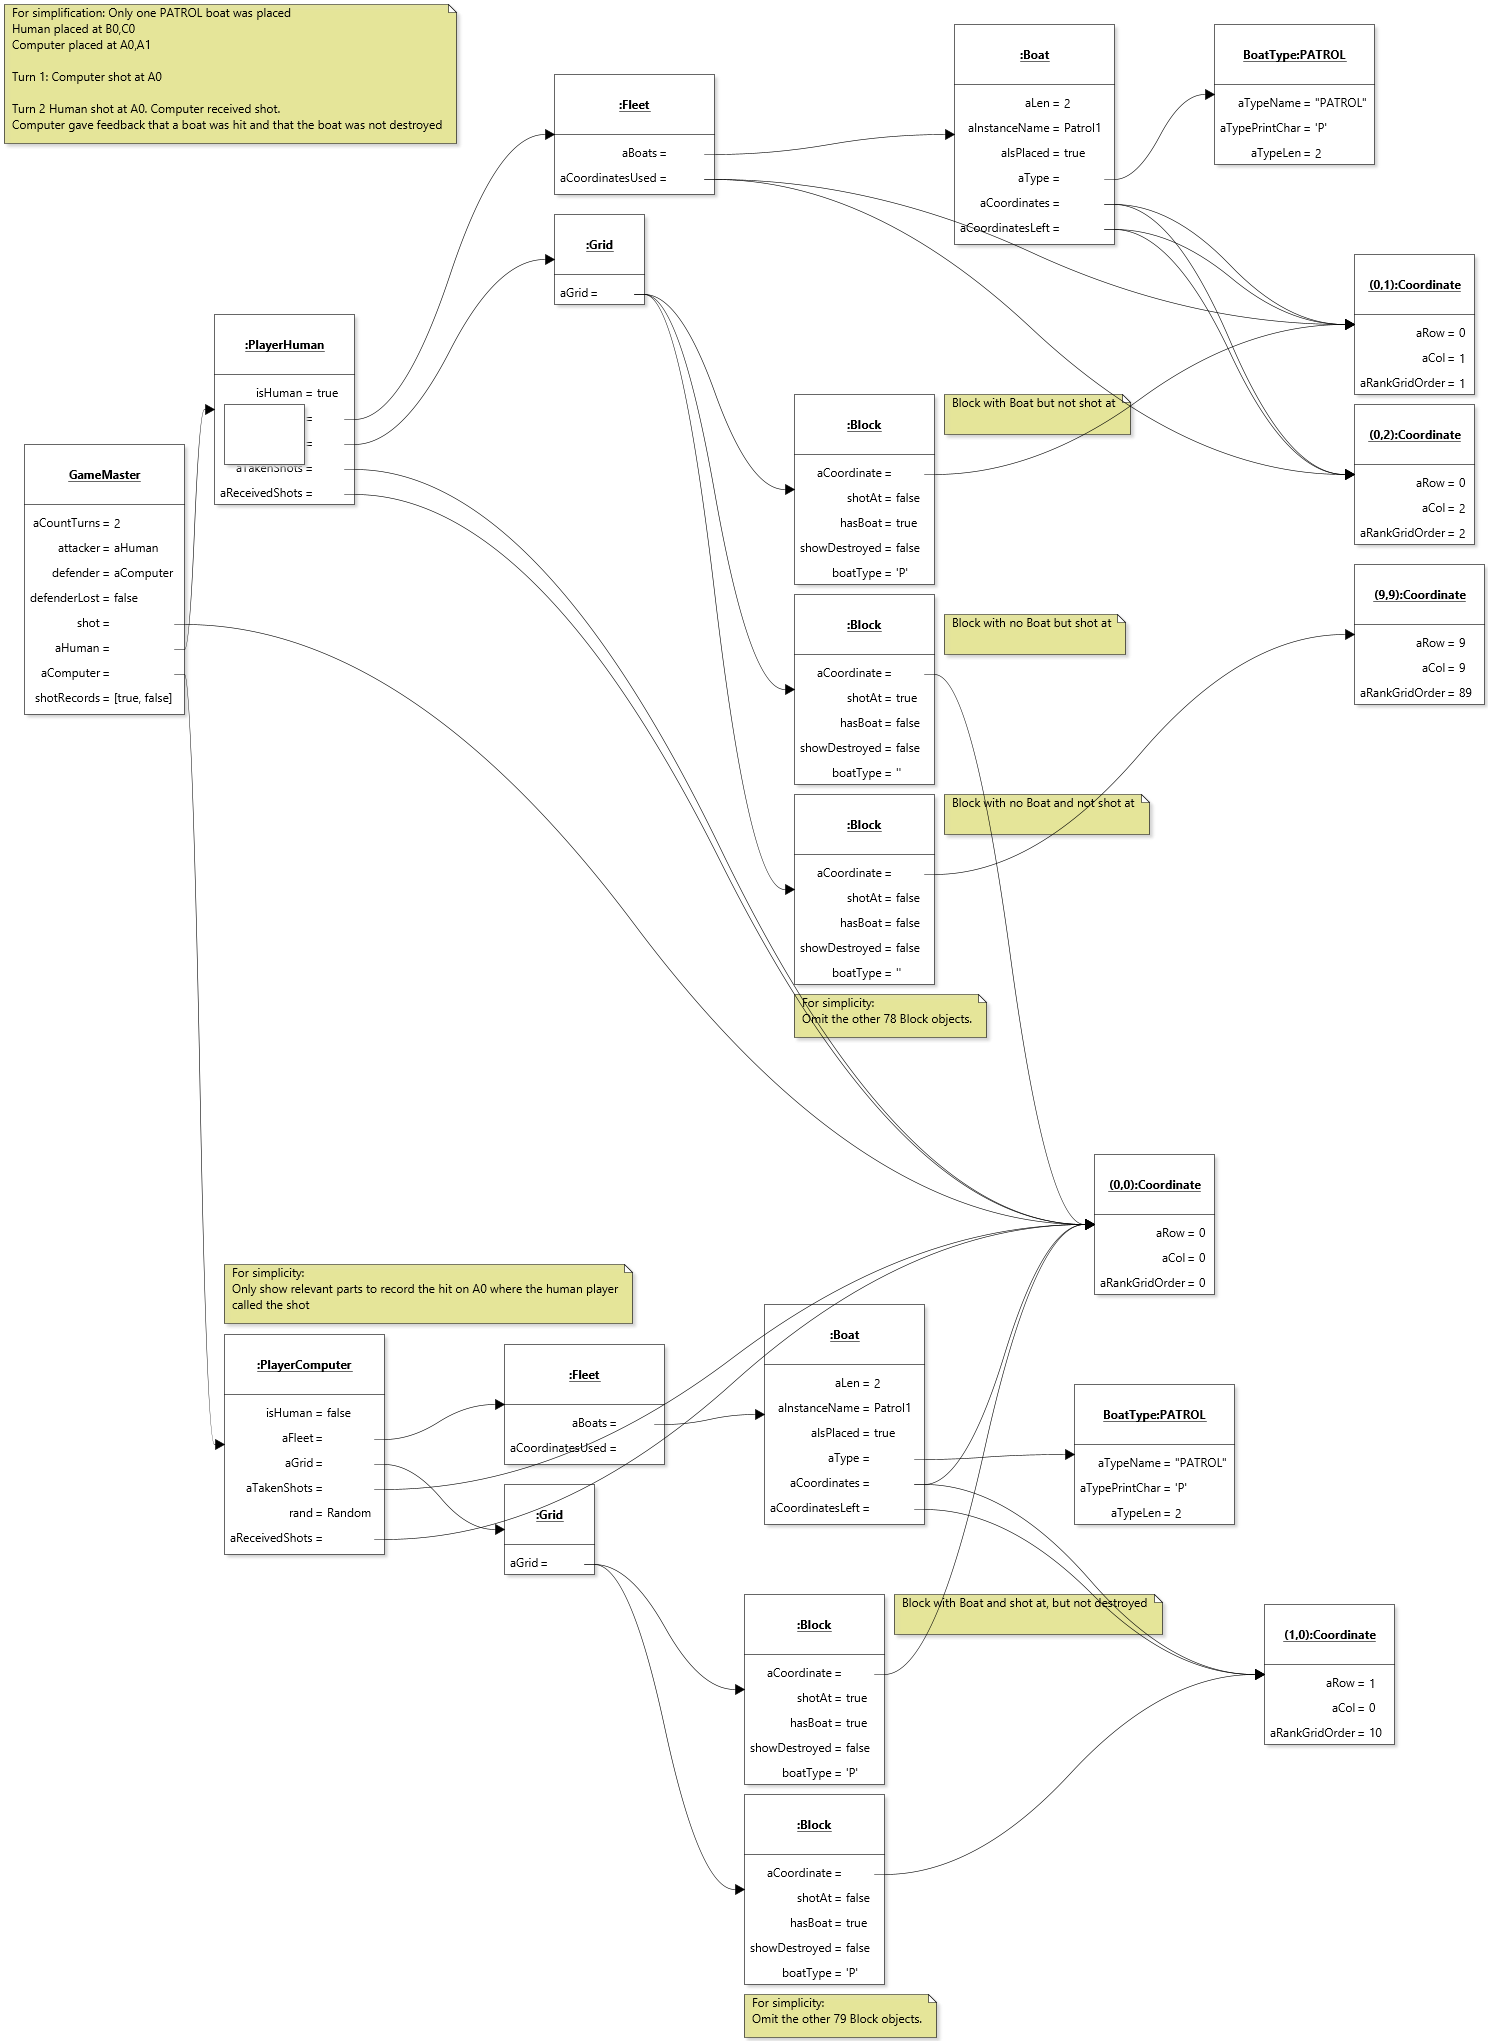
\includegraphics[width = 0.9\linewidth]{images/object_diagram.png}
\caption{Object diagram including Coordinate objects}
\end{figure}

\begin{figure}[h]
\centering
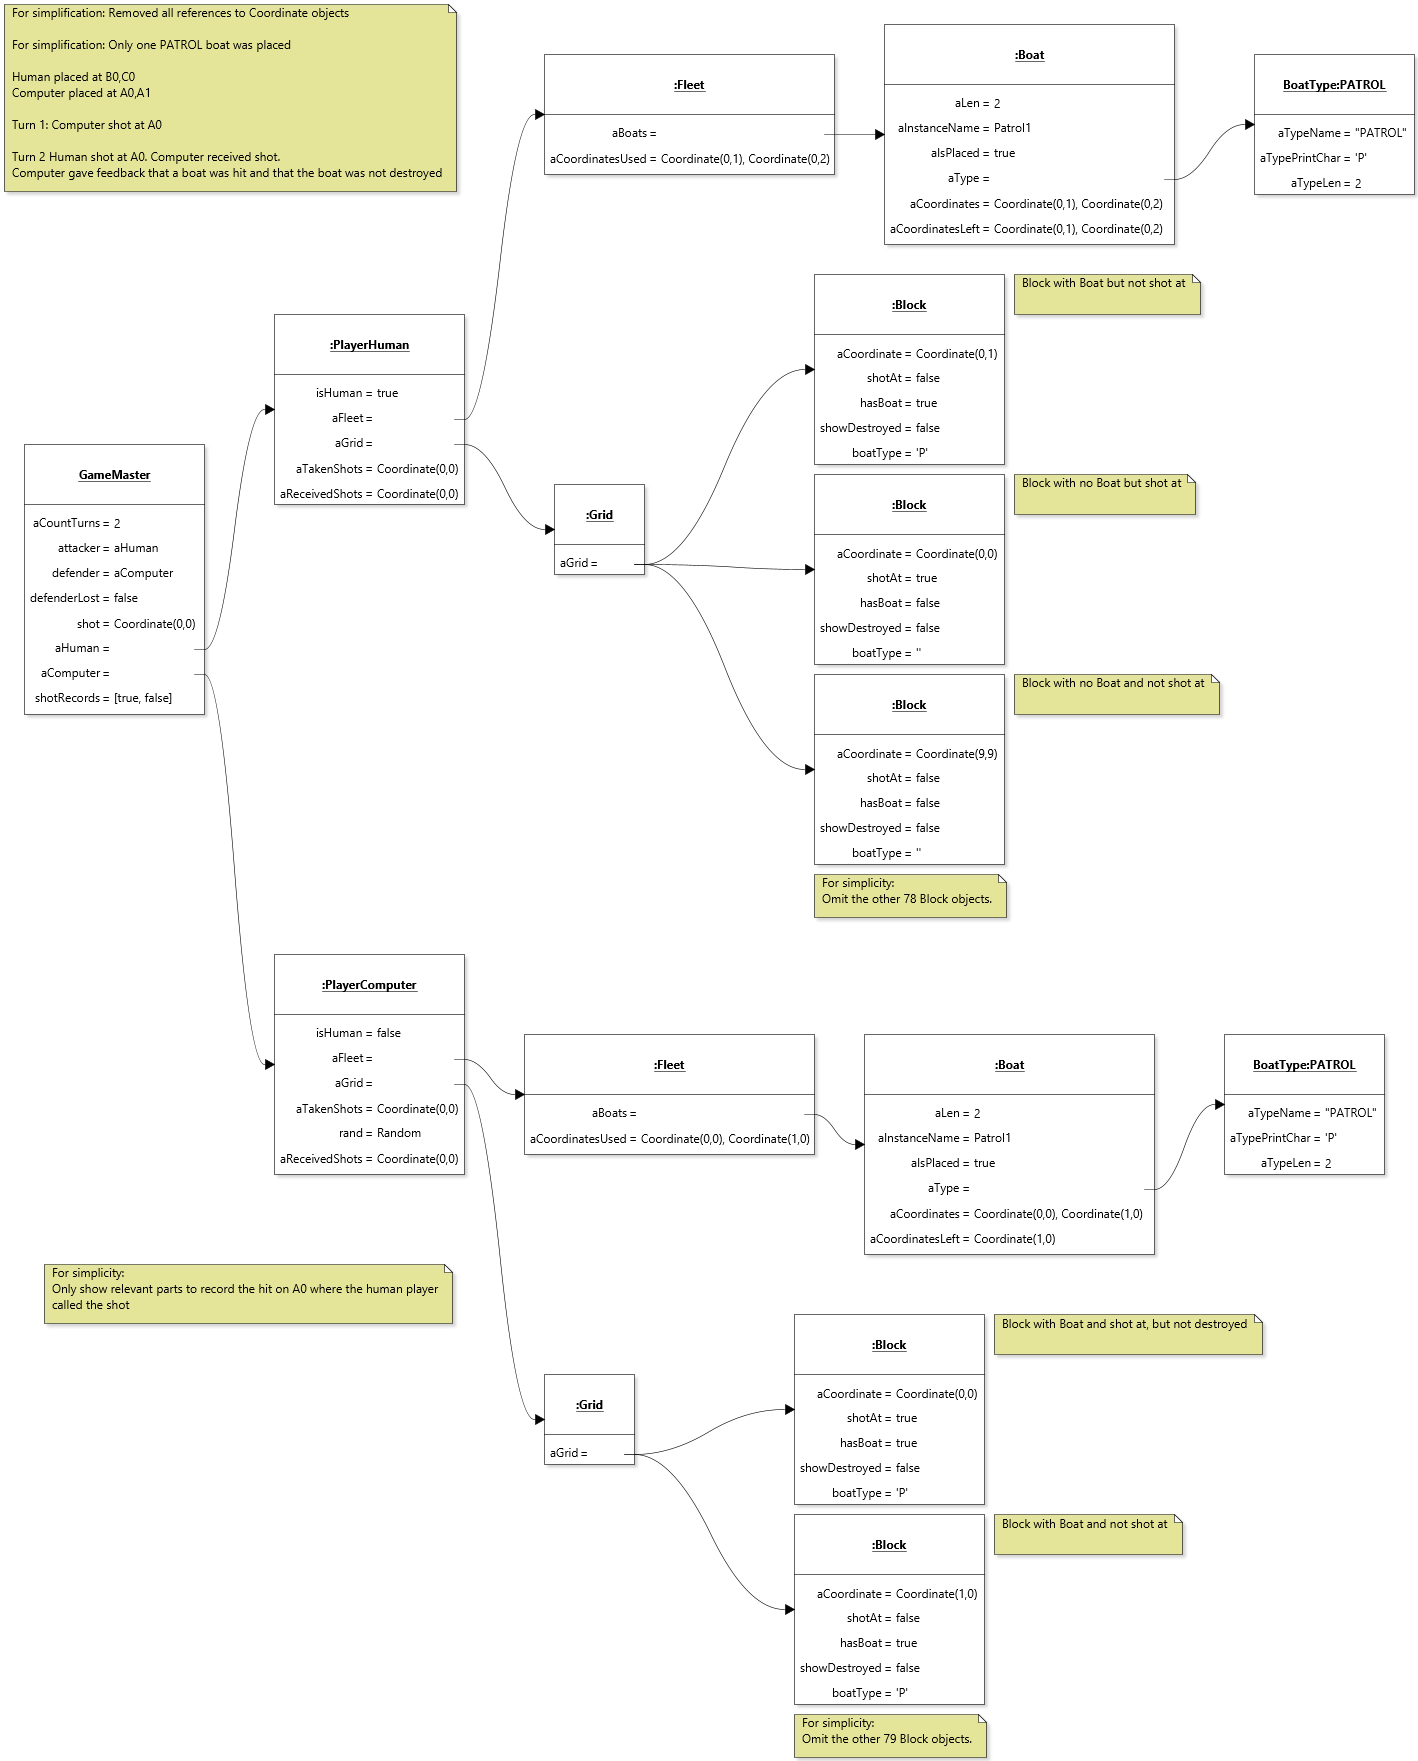
\includegraphics[width = \linewidth]{images/object_diagram_simplified.png}
\caption{Object diagram without the Coordinate objects}
\end{figure}



\end{document}
